% This text is proprietary.
% It's a part of presentation made by myself.
% It may not used commercial.
% The noncommercial use such as private and study is free
% Sep. 2005 
% Author: Sascha Frank 
% University Freiburg 
% www.informatik.uni-freiburg.de/~frank/

\documentclass{beamer}
\usepackage{multicol}
\usepackage{amsmath}

\usetheme{Warsaw}

\begin{document}
\title{RSA Public and Private Key Generation}   
\author{Jason Pearson and Sam Demorest} 
\date{\today} 

\frame{\titlepage} 

%\frame{
%	\frametitle{Overview}\tableofcontents
%}  

\frame{\frametitle{Design Decisions}
	Used the in beta programming language Rust\newline
	Two separate programs reuse-ability\newline
	Public and private key generation\newline
	Encryption and decryption of characters\newline	
}

\frame{\frametitle{Implimentation}
	Miller-Rabin instead of AKS for speed\newline
	Modular exponentiation\newline
	ASCII representation of character for encrypting\newline
	Used an inverse function instead of Extended Euclidean Elgorithm\newline
}

\frame{\frametitle{Output}
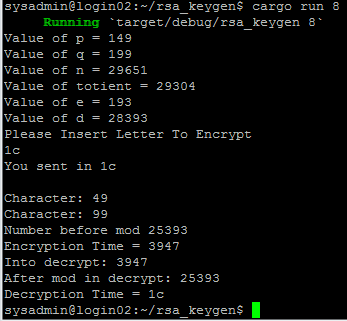
\includegraphics[scale=0.8]{Capture.png}
}

\frame{\frametitle{Conclusion}
	Able to determine large prime numbers\newline
	Able to encrypt one character and decrypt it\newline \newline
	BigInt library not fully ready for deployment yet \newline
	No use of bit twiddling operations for optimization \newline
}

\frame{\frametitle{Demo!}
	Demo Time!\newline
}


\frame{\frametitle{References}
	
	AKS References:\newline
	http://www.cse.iitk.ac.in/users/manindra/algebra/primality\_v6.pdf\newline
	http://mathworld.wolfram.com/AKSPrimalityTest.html\newline
	
	Rust References:\newline
	https://doc.rust-lang.org/\newline
	http://rustbyexample.com/\newline
	https://github.com/rust-lang/rust\newline
	
	RSA Cryptosystem References:\newline
	http://mathworld.wolfram.com/RSAEncryption.html\newline
	https://engineering.purdue.edu/kak/compsec/NewLectures/Lecture12.pdf\newline
	
}
\end{document}

